\chapter{Organisation}

Dieses Kapitel beschreibt kurz die Stakeholder des Projekts sowie den allgemeinen Aufbau.

\section{Projektbeteiligte}

\begin{table}[H]
	\centering
	\begin{tabular}{p{0.3\textwidth} p{0.2\textwidth} p{0.3\textwidth}}
	\textbf{Name} & \textbf{Funktion} & \textbf{E-Mail Adresse} \\ \midrule
	Simon Meer & Student & simon.meer@students.bfh.ch \\
	Prof. Urs K�nzler & Betreuer & urs.kuenzler@bfh.ch \\
	Yves Petitpierre & Experte & yves.petitpierre@ericsson.com \\
	\end{tabular}
\end{table}

\section{Projektmanagement}

Meetings zwischen dem Studenten und dem Betreuer finden jeden zweiten Mittwoch in Biel statt.

Das Projekt wird innerhalb eines Git-Projektes gef�hrt und im Laufe des Projekts entweder auf GitHub.com oder auf das interne Projektmanagement-Tool migriert.

Gearbeitet wird durch den Studenten Montags bis Donnerstags an einem Arbeitsplatz im CPVR Labor in Biel.

\begin{sidewaysfigure}
	\section{Ordnerstruktur}
	
	\centering
	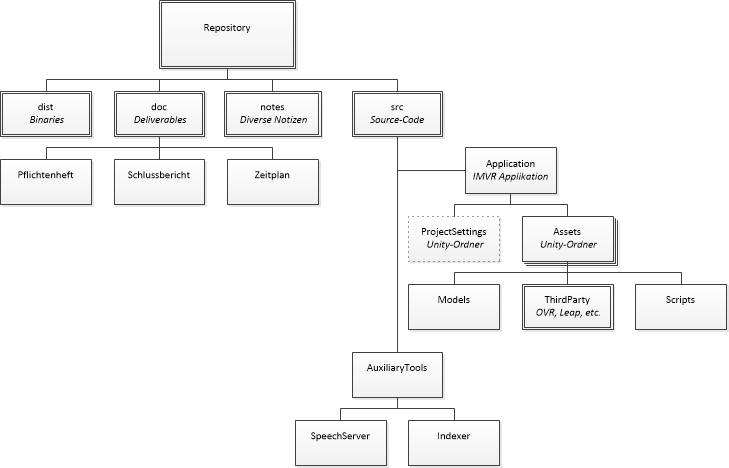
\includegraphics{bilder/file_structure}
	\caption{Die Ordnerstruktur des Projektes.}
\end{sidewaysfigure}

\section{Zeitplan}

